\documentclass[aspectratio=169,xcolor={dvipsnames,table}]{beamer}
\usepackage[no-math,deluxe,haranoaji]{luatexja-preset}
\renewcommand{\kanjifamilydefault}{\gtdefault}
\renewcommand{\emph}[1]{{\upshape\bfseries #1}}
\usetheme{metropolis}
\metroset{block=fill}
\setbeamertemplate{navigation symbols}{}
\setbeamertemplate{blocks}[rounded][shadow=false]
\usecolortheme[rgb={0.7,0.2,0.2}]{structure}
%%%%%%%%%%%%%%%%%%%%%%%%%%
%% Change alert block colors
%%% 1- Block title (background and text)
\setbeamercolor{block title alerted}{fg=mDarkTeal, bg=mLightBrown!45!yellow!45}
\setbeamercolor{block title example}{fg=magenta!10!black, bg=mLightGreen!70}
%%% 2- Block body (background)
\setbeamercolor{block body alerted}{bg=mLightBrown!25}
\setbeamercolor{block body example}{bg=mLightGreen!15}
%%%%%%%%%%%%%%%%%%%%%%%%%%%

\usepackage[absolute,overlay]{textpos}  %% 任意の位置に図を配置
%\usepackage[grid=true,gridcolor=Maroon,subgridcolor=gray,gridunit=pt,texcoord]{eso-pic} %%場所決めのための格子
%%%%%%%%%%%%%%%%%%%%%%%%%%%
%% さまざまなアイコン
%%%%%%%%%%%%%%%%%%%%%%%%%%%
%\usepackage{fontawesome}
\usepackage{fontawesome5}
\usepackage{figchild}
\usepackage{twemojis}
\usepackage{utfsym}
\usepackage{bclogo}
\usepackage{marvosym}
\usepackage{fontmfizz}
\usepackage{pifont}
\usepackage{phaistos}
\usepackage{worldflags}
\usepackage{jigsaw}
\usepackage{tikzlings}
\usepackage{tikzducks}
\usepackage{scsnowman}
\usepackage{epsdice}
\usepackage{halloweenmath}
\usepackage{svrsymbols}
\usepackage{countriesofeurope}
\usepackage{tipa}
%%%%%%%%%%%%%%%%%%%%%%%%%%%
\usepackage{tikz}
\usetikzlibrary{calc,patterns,decorations.pathmorphing,backgrounds}
\usepackage{tcolorbox}
\usepackage{tikzpeople}
\usepackage{circledsteps}
\usepackage{xcolor}
\usepackage{amsmath}
\usepackage{booktabs}
\usepackage{chronology}
\usepackage{signchart}
%%%%%%%%%%%%%%%%%%%%%%%%%%%
%% 場合分け
%%%%%%%%%%%%%%%%%%%%%%%%%%%
\usepackage{cases}
%%%%%%%%%%%%%%%%%%%%%%%%%%
\usepackage{pdfpages}
%%%%%%%%%%%%%%%%%%%%%%%%%%%
%% 音声リンク表示
\newcommand{\myaudio}[1]{\href{#1}{\faVolumeUp}}
%%%%%%%%%%%%%%%%%%%%%%%%%%
%% \myAnch{<名前>}{<色>}{<テキスト>}
%% 指定のテキストを指定の色の四角枠で囲み, 指定の名前をもつTikZの
%% ノードとして出力する. 図には remember picture 属性を付けている
%% ので外部から参照可能である.
\newcommand*{\myAnch}[3]{%
  \tikz[remember picture,baseline=(#1.base)]
    \node[draw,rectangle,line width=1pt,#2] (#1) {\normalcolor #3};
}
%%%%%%%%%%%%%%%%%%%%%%%%%%
%% \myEmph コマンドの定義
%%%%%%%%%%%%%%%%%%%%%%%%%%
%\newcommand{\myEmph}[3]{%
%    \textbf<#1>{\color<#1>{#2}{#3}}%
%}
\usepackage{xparse} % xparseパッケージの読み込み
\NewDocumentCommand{\myEmph}{O{} m m}{%
    \def\argOne{#1}%
    \ifx\argOne\empty
        \textbf{\color{#2}{#3}}% オプション引数が省略された場合
    \else
        \textbf<#1>{\color<#1>{#2}{#3}}% オプション引数が指定された場合
    \fi
}
%%%%%%%%%%%%%%%%%%%%%%%%%%%
%%%%%%%%%%%%%%%%%%%%%%%%%%%
%% 文末の上昇イントネーション記号 \myRisingPitch
%% 通常のイントネーション \myDownwardPitch
%% https://note.com/dan_oyama/n/n8be58e8797b2
%%%%%%%%%%%%%%%%%%%%%%%%%%%
\newcommand{\myRisingPitch}{
\begin{tikzpicture}[scale=0.3,baseline=0.3]
\draw[->,>=stealth] (0,0) to[bend right=45] (1,1);
\end{tikzpicture}
}
\newcommand{\myDownwardPitch}{
\begin{tikzpicture}[scale=0.3,baseline=0.3]
\draw[->,>=stealth] (0,1) to[bend left=45] (1,0);
\end{tikzpicture}
}
%%%%%%%%%%%%%%%%%%%%%%%%%%%%
%\AtBeginSection[%
%]{%
%  \begin{frame}[plain]\frametitle{授業の流れ}
%     \tableofcontents[currentsection]
%   \end{frame}%
%}

\usetikzlibrary{tikzmark}
%%%%%%%%%%%%%%%%%%%%%%%%%%
%%%%%%%%%%%%%%%%%%%%%%%%%%%
\title{English is fun.}
\subtitle{Sleeping is necessary to us.}
\author{}
\institute[]{}
\date[]

%%%%%%%%%%%%%%%%%%%%%%%%%%%%
%% TEXT
%%%%%%%%%%%%%%%%%%%%%%%%%%%%
\begin{document}

\begin{frame}[plain]
  \titlepage
\end{frame}

\section*{授業の流れ}
\begin{frame}[plain]
  \frametitle{授業の流れ}
  \tableofcontents
\end{frame}

%%%%%%%%%%%%%%%%%%%%%%%%%%%%%%%%%%%%%%%%%%%%
\section{動名詞}
%%%%%%%%%%%%%%%%%%%%%%%%%%%%%%%%%%%%%%%%%%%%%
\begin{frame}[plain]{~すること}
 \large

\begin{enumerate}
 \item<1-> Exercise is good for your health.\hfill{\scriptsize exercise \textipa{/\'eks@s\`aIz/} 運動 health \textipa{/h\'elT/} 健康}
 \item<2-> \alt<3->{\fbox{To eat vegetables}}{To eat vegetables} is good for your health.\hfill\visible<4->{\scriptsize 不定詞の名詞的用法}
 \item<5-> \alt<6->{\fbox{Eating vegetables}}{Eating vegetables} is good for your health.\hfill\visible<7->{{\scriptsize \fbox{Eating vegetables} $=$ S}}
 \item<8-> His job is \alt<9->{\fbox{helping students}}{helping students}.\hfill\visible<10->{{\scriptsize His job $=$ \fbox{helping students}}}
\end{enumerate}

\begin{block}{Topics for Today}
\begin{itemize}\setbeamertemplate{items}[square]\small
 \item<11->   \Circled[fill color= white]{\,\,--ing\,\,} が「~すること」という意味を表し、名詞のはたらきをすることがある%
\hfill{\tiny 0210}\,{\scriptsize \myaudio{./audio/036_gerund_01.mp3}}
\item <12-> 名詞のはたらきをする \Circled[fill color= white]{\,\,--ing\,\,}\,を「動名詞」といいます
\item<13-> \Circled[fill color= white]{\,\,--ing\,\,}\,が
      \begin{itemize}\setbeamertemplate{items}[circle]\small
       \item 文全体の主語になったり
       \item be動詞の直後にきたりすることがあります
      \end{itemize}
 
 \end{itemize}
     \end{block}
\end{frame}
%%%%%%%%%%%%%%%%%%%
\begin{frame}[plain]{Exercises}

{\small (~~~~~~)内から正しいものを選びましょう}%
\hfill{\tiny 0140}\,{\scriptsize \myaudio{./audio/036_gerund_02.mp3}}
 \begin{enumerate}
  \item ( Play / \alt<2->{\Circled[outer color = BurntOrange]{ Playing }}{~~Playing~~} ) the guitar is one of my hobbies.\hfill{\scriptsize hobbies: hobby(趣味)の複数形}
  \item ( Play / Run / \alt<3->{\Circled[outer color = BurntOrange]{ Eating }}{~~Eating~~} ) outside  is fun.\hfill{\scriptsize outside \textipa{/aUts\`aId/} 室外で}
  \item Her job is ( drive / \alt<4->{\Circled[outer color = BurntOrange]{ driving }}{~~driving~~} ) a bus.
 \end{enumerate}
\end{frame}
%%%%%%%%%%%%%%%%%%%%%%
\begin{frame}[plain]{Exercises}

{\small 日本文の意味になるように(~~~~~)内の語句を並べ替えましょう。先頭にくる語は大文字で書きはじめてください}%
\hfill{\tiny 0204}{\scriptsize \myaudio{./audio/036_gerund_03.mp3}}
 \begin{enumerate}
  \item {\small 走ることは健康にいい。}\hfill{\scriptsize be good for 〜にいい}\\
	( your health / is / good / running / for ).\\
	\visible<2->{Running is good for your health.\hfill{\scriptsize running: nが重なることに注意}}
  \item {\small 川で泳ぐことは楽しい。}\\
	( the river / fun / swimming / is / in ).\\
	\visible<3->{Swimming in the river is fun.\hfill{\scriptsize swimming: mが重なることに注意}}
  \item {\small 私のお気に入りの趣味は読書です。}\hfill{\scriptsize favorite \textipa{/f\'eIv@rIt/ お気に入りの}}\\
	My ( reading / hobby / is / favorite ).\\
	\visible<4->{My favorite hobby is reading.}
  \item {\small 彼女の仕事はバスを運転することだ。}
	Her ( driving / job / a bus / is ).\\
	\visible<5->{Her job is driving a bus.\hfill{\scriptsize driving: driveのeが落ちることに注意}}
 \end{enumerate}
\end{frame}
%%%%%%%%%%%%%%%%%%%%%%%%%%%%%%%%%%%%%%%%
\section{V $+$ --ing}
\begin{frame}[plain]{V $+$ --ing}
 \begin{enumerate}
  \item<1-> He started \fbox{his business} two years ago.\hfill{\scriptsize start \textipa{/st\'A\textrhookschwa t/} 始める}\\
\hspace{80pt}\visible<2->{{($=$ O)}}\hfill{\scriptsize business \textipa{/b\'Izn@s/} 商売}
  \item<3-> He started \alt<4->{\fbox{to laugh}}{to laugh}\,.\hfill{\scriptsize laugh \textipa{/l\'\ae f/} 笑う}
  \item<5-> He started \alt<6->{\fbox{laughing}}{laughing}\,.%
\hfill\visible<7->{{\scriptsize \fbox{laughing} $=$ \textbf{O}}}
 \end{enumerate}

\vspace{20pt}

\begin{block}<8->{Topic for Today}
\begin{itemize}\setbeamertemplate{items}[square]\small
 \item \Circled[fill color= white]{\,\,--ing\,\,}\,\,が、「〜すること」の意味で、目的語になることがあります
 \end{itemize}
     \end{block}

\hfill{\tiny 0138}\,{\scriptsize \myaudio{./audio/036_gerund_04.mp3}}

\end{frame}
%%%%%%%%%%%%%%%%%%%%%%%%%%%%
%\begin{frame}[plain]{Exercises}
% \begin{enumerate}
%  \item \begin{enumerate}
%	 \item<1-> She likes music.
%	 \item<2-> She likes \alt<3->{\fbox{to play the piano}}{to play the piano}.
%	 \item<4-> She likes \alt<5->{\fbox{playing the piano}}{playing the piano}.      
%	\end{enumerate}
%  \item \begin{enumerate}
%	 \item<6-> They began the lesson.
%	 \item<7-> They began \alt<8->{\fbox{to study English}}{to study English}.
%	 \item<9-> They began \alt<10->{\fbox{studying English}}{studying English}.
%	\end{enumerate}
% \end{enumerate}
%\end{frame}
%%%%%%%%%%%%%%%%%%%%%%%%%%%%%
\begin{frame}[plain]{Exercises}

{\small 日本語の意味になるよう(~~~~~~~~)内の語句を並べ替えましょう。ただし不要な語が1語含まれています}%
\hfill{\tiny 0139}\,{\scriptsize \myaudio{./audio/036_gerund_05.mp3}}
\begin{enumerate}
 \item {\small 雨がふり始めました。}\\
       It ( began / begin / raining ).\\
       \visible<2->{It began raining. (× begin)}
 \item {\small ジョージはその本を読み始めた。}\\
       George ( book / read / reading / the / started ).\\
       \visible<3->{George started reading the book. (× read)} 
 \item {\small 彼は家族に夕食を作るのが好きです。}\\
       He ( dinner / his family / likes / for / make / cooking ).\\
       \visible<4->{He likes cooking dinner for his family. (× cook)}
\end{enumerate}
\end{frame}
%%%%%%%%%%%%%%%%%%%%%%%%%%%%%%%%%
\section{動名詞とto不定詞}
\begin{frame}[plain,t]{動名詞とto不定詞}

\begin{enumerate}
 \item<1-> \begin{enumerate}
	\item To speak English is difficult for me.
	\item (\alt<2->{~~Speaking~~}{\phantom{~~Speaking~~}}) English is difficult for me.%
\hspace{51pt}\visible<3->{{\scriptsize Speaking English $=$ To speak English}}
       \end{enumerate}
 \item<4->  \begin{enumerate}
	\item Her job is to help students.
	\item Her job is (\alt<5->{~~helping~~}{\phantom{~~helping~~}}) students.%
\hfill\visible<6->{{\scriptsize Helping students $=$ To help students}}
       \end{enumerate}
 \item<7-> \begin{enumerate}
	\item I love to sing.
	\item I love (\alt<8->{~~singing~~}{\phantom{~~singing~~}}).%
\hspace{146pt}\visible<9->{{\scriptsize singing $=$ to sing}}

       \end{enumerate}
\end{enumerate}

\vspace{53pt}

\begin{block}<10->{Topic for Today}
\begin{itemize}\setbeamertemplate{items}[square]\small
 \item  動名詞と「名詞的用法のto不定詞」は、「〜すること」という意味で名詞として働く点で同じです
\end{itemize}
     \end{block}

\vspace{-15pt}

\hfill{\tiny 0238}\,{\scriptsize \myaudio{./audio/036_gerund_06.mp3}}

\begin{textblock*}{0.4\linewidth}(355pt,97pt)
\visible<11->{\begin{tikzpicture}
\pig[
signpost=\scalebox{0.5}{
\parbox{2.2cm}{\color{black}
\centering ---ing $=$ to ---\\おなじ!}},
signcolour= brown!70!gray,
signback=white!80!brown
]
\end{tikzpicture}}
\end{textblock*}


\end{frame}
%%%%%%%%%%%%%%%%%%%%%%%%%%%%%%%%
\begin{frame}[plain]{動名詞しか使えない場合}

 \begin{enumerate}
  \item \begin{enumerate}
	 \item<1-> She began reading the book.\hfill{\scriptsize began \textipa{/bIg\'\ae n/} 始めた}
	 \item<2-> She began to read the book.
	\end{enumerate}
  \item \begin{enumerate}
	 \item<4-> She \myEmph[4-]{Maroon}{finished} read\myEmph[4-]{Maroon}{ing} the book.\hfill{\scriptsize finish \textipa{/f\'InIS/} 終える}
	 \item<5-> *She finished to read the book.
	\end{enumerate}
  \item \begin{enumerate}
	 \item<7-> He \myEmph[7-]{Maroon}{enjoyed} read\myEmph[7-]{Maroon}{ing} the book.\hfill{\scriptsize enjoy \textipa{/IndZ\'OI/} 楽しむ}
	 \item<8-> *He enjoyed to read the book.
	\end{enumerate}
 \end{enumerate}
%
\hfill{\tiny 0156}\,{\scriptsize \myaudio{./audio/036_gerund_07.mp3}}

\begin{block}<3->{Topics for Today}
\begin{itemize}\setbeamertemplate{items}[square]\small
 \item<3->  動名詞と「名詞的用法のto不定詞」は、「〜すること」の意味で名詞として働く点で同じです
 \item<6-> でも、目的語のとき動名詞しか使えない場合があります \dbend
       \begin{itemize}\setbeamertemplate{items}[circle]\small
	\item<6-> \textbf{finish ---ing}(〜し終える)\hfill{}*finish to ---
	\item<9-> \textbf{enjoy ---ing}(〜するのを楽しむ)\hfill{}*enjoy to ---
       \end{itemize}
 \end{itemize}
     \end{block}
\end{frame}
%%%%%%%%%%%%%%%%%%%%%%%%%%%%%
\begin{frame}[plain,t]{Exercises}

{\small (~~~~~~)内から正しいものを選びましょう}%
\hfill{\tiny 0156}\,{\scriptsize \myaudio{./audio/036_gerund_08.mp3}}
 \begin{enumerate}
  \item Do you like ( cook / \alt<2->{\Circled[outer color = BurntOrange]{ cooking }}{~~cooking~~} ) ?
  \item Do you like ( cook / \alt<3->{\Circled[outer color = BurntOrange]{ to  cook }}{~~to cook~~} ) ?
  \item He enjoyed ( play / \alt<4->{\Circled[outer color = BurntOrange]{ playing }}{~~playing~~} / to play ) golf.
  \item She finished ( write / \alt<5->{\Circled[outer color = BurntOrange]{ writing }}{~~writing~~} / to write ) a letter.
 \end{enumerate}

\begin{textblock*}{0.4\linewidth}(315pt,150pt)
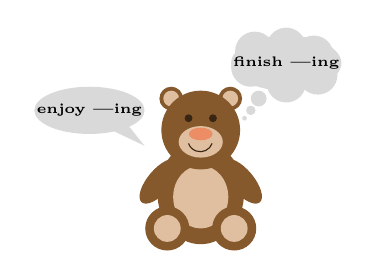
\begin{tikzpicture}
\bear[
speech={\tiny\bfseries enjoy ---ing},
think={\tiny\bfseries finish ---ing},
bubblecolour=gray!30!white
]
\end{tikzpicture}
\end{textblock*}
\end{frame}
%%%%%%%%%%%%%%%%%%%%%%%%%%%%%%%%%%%%%%%%
\section{動名詞のまとめ}
%%%%%%%%%%%%%%%%%%%%%%%%%%%%%%%%%%%%%%%%
\begin{frame}[plain]{要点1}

\begin{block}{動名詞の基礎}
\begin{itemize}\setbeamertemplate{items}[square]\small
 \item<2->   \Circled[fill color= white]{\,\,--ing\,\,} が「~すること」という意味を表し、名詞のはたらきをすることがある%
 \item<3-> 名詞のはたらきをする \Circled[fill color= white]{\,\,--ing\,\,}\,を「動名詞」といいます
 \item<4-> \Circled[fill color= white]{\,\,--ing\,\,}\,が
      \begin{itemize}\setbeamertemplate{items}[circle]\small
       \item<5-> 文全体の主語になったり\hfill{\scriptsize \fbox{\textbf{Eating} vegetables} is good for your health.}\\
\hfill\visible<8->{{\scriptsize $=$ \fbox{\textbf{To eat} vegetables} is good for your health.}}
       \item<6-> be動詞の直後にきたり\hfill{\scriptsize His job is \fbox{\textbf{helping} students}.}\\
\hfill\visible<9->{{\scriptsize $=$ His job is \fbox{\textbf{to help} students}.}}
       \item<7-> 目的語になることがあります\hfill{\scriptsize She started \fbox{\textbf{singing}}}.\\
\hfill\visible<10->{{\scriptsize $=$ She started \fbox{\textbf{to sing}}.}}
      \end{itemize}
 \end{itemize}
     \end{block}
\hfill\visible<11->{{\scriptsize 動名詞と「名詞的用法のto不定詞」は、「〜すること」の意味で名詞として働く点で同じです}}
\end{frame}
%%%%%%%%%%%%%%%%%%%%%%%%%%%%%%%%%%%%%%%%
\begin{frame}[plain]{要点2}

\begin{block}{動名詞とto不定詞}
\begin{itemize}\setbeamertemplate{items}[square]\small
 \item  動名詞と「名詞的用法のto不定詞」は、「〜すること」の意味で名詞として働く点で同じです
 \item でも、動名詞しか使えない場合があります \dbend
       \begin{itemize}\setbeamertemplate{items}[circle]\small
	\item \textbf{finish ---ing}(〜し終える)\hfill{\scriptsize She \textbf{finished reading} the book.}\\
\hfill{{\scriptsize *She finished to read the book.}}
	\item \textbf{enjoy ---ing}(〜するのを楽しむ)\hfill{\scriptsize They \textbf{enjoyed playing} tennis.}\\
\hfill{{\scriptsize *They enjoyed to play tennis.}}
       \end{itemize}
\hfill{}ほかにもありますが、まずは\textbf{finish}と\textbf{enjoy}を覚えましょう!
 \end{itemize}
     \end{block}
\end{frame}
%%%%%%%%%%%%%%%%%%%%%%%%%%%%%%%%%%%%%%%%
\section{2つのbe $+$ ---ing}
%%%%%%%%%%%%%%%%%%%%%%%%%%%%%%%%%%%%%%%%
\begin{frame}[plain,t]{2つのbe $+$ ---ing}

 \begin{enumerate}
  \item<1-> Her hobby is \tikzmark{ing1}listening to the radio.%
\hfill\visible<3->{{\scriptsize Her hobby $=$ \fbox{listening to the radio}}}\\
\hfill\visible<4->{{\scriptsize \tikzmark{gerund}このlisteningは動名詞}}\\
\hfill\visible<5->{{\scriptsize *Her hobby listens to the radio.}}
  \item<2-> She is \tikzmark{ing2}listening to the radio.\visible<7->{{\scriptsize (現在進行形)}}\hfill\visible<6->{{\scriptsize $<$ She listens to the radio.(現在形)}}\\
\hfill\visible<8->{{\scriptsize \tikzmark{participle}このlisteningは現在分詞}}\\

 \end{enumerate}
%

\vspace{70pt}

\begin{block}<9->{S $+$ be $+$ ---ing}\small
 \begin{enumerate}\setbeamertemplate{items}[circle]
  \item<10-> S $=$ 動名詞\hspace{29pt}$\rightarrow$\hspace{5pt}S $+$ be $+$ ---ing($=$ 動名詞)\hfill{}「Sは~することだ」
  \item<11-> S $+$ V. の進行形\hspace{10pt}$\rightarrow$\hspace{5pt}S $+$ be $+$ ---ing($=$ 現在分詞)\hfill{}「Sは~している」
 \end{enumerate}
\end{block}

\vspace{-15pt}

\hfill{\tiny 0117}\,{\scriptsize \myaudio{./audio/036_gerund_09.mp3}}

\begin{textblock*}{0.4\linewidth}(335pt,120pt)
\begin{tikzpicture}
\duck[signpost=\scalebox{0.3}{
\parbox{2.5cm}{\color{black}
動名詞?\\現在分詞?}},
signcolour=brown!70!gray,
signback=white!80!brown,
graduate=gray!20!black,
tassel=red!70!black,
speech={\tiny きちんと区別}
]
\end{tikzpicture}
\end{textblock*}


\begin{tikzpicture}[remember picture,overlay]
% \visible<4->{\draw[<-,opacity=.4,line width=1pt] ([xshift=22pt,yshift=-4pt]pic cs:ing1) to[out=-20, in=190] ([xshift=-2pt, yshift=2pt] pic cs:gerund);}
% \visible<8->{\draw[<-,opacity=.4,line width=1pt] ([xshift=22pt,yshift=-4pt]pic cs:ing2) to[out=-20,in=190] ([xshift=-2pt, yshift=2pt] pic cs:participle);}
%%%%%%%%%%%%%%%%%
% Calculate intermediate points
  \coordinate (A1) at ($(pic cs:ing1) + (22pt,-13pt)$); % 10pt below ing1
  \coordinate (A2) at ($(pic cs:ing2) + (22pt,-13pt)$); % 10pt below ing1
  % Draw the arrow with right angles
  \visible<4->{\draw[<-,Maroon,line width=1pt] ([xshift=22pt,yshift=-2pt]pic cs:ing1) -- (A1) -- ([xshift=-2pt,yshift=2pt]pic cs:gerund);}
  \visible<8->{\draw[<-,Maroon,line width=1pt] ([xshift=22pt,yshift=-2pt]pic cs:ing2) -- (A2) -- ([xshift=-2pt,yshift=2pt]pic cs:participle);}
%%%%%%%%%%%
\end{tikzpicture}
\end{frame}
%%%%%%%%%%%%%%%%%%%%%%%%%%%%%
\begin{frame}[plain]{Exercises}
 
{\small 各英文の意味を考えましょう}%
\hfill{\tiny 0349}\,{\scriptsize \myaudio{./audio/036_gerund_10.mp3}}


\begin{enumerate}
 \item His job is teaching English.
 \item He is teaching English.
 \item Our plan is going to the park tomorrow.
 \item Her goal is learning a new language.\hfill{\scriptsize goal \textipa{/g\'oUl/ 目標}}
 \item She is learning a new language.
 \item Their dream is winning the game.\hfill{\scriptsize win the game: 試合に勝つ}
 \item My hobby is collecting stamps.\hfill{\scriptsize collect \textipa{/k@l\'ekt/} 集める stamp \textipa{/st\'\ae mp/} 切手}
 \item She is collecting old coins.\hfill{\scriptsize coin \textipa{/k\'OIn/ 硬貨}}
\end{enumerate}
\end{frame}
%%%%%%%%%%%%%%%%%%%%%%
\end{document}

